\chapter{Synthetic Data}\label{chap:synthetic_data}

There are many scenarios where privacy preserving machine learning is desirable. For instance, consider a dataset which contains patient data, such as their health history. A leak of this dataset would be very bad for the patient's privacy, as the disclosed information could be used to discriminate against them (e.g. higher health insurance premiums). This risk can make patients more hesitant to share their data. This in turn causes the problem of having small datasets. 

In the cyber risk scenario, historical data is lacking. This is because many insurance companies have just started to offer this line of product. While we were able to get a few anonymised cyber insurance questionnaires from our industry partner\footnote{\href{https://zisc.ethz.ch/research/projects/privacy-preserving-machine-learning-for-cyber-insurance/}{https://zisc.ethz.ch/research/projects/privacy-preserving-machine-learning-for-cyber-insurance/}}, it is not enough to properly evaluate our model. This is the motivation of this chapter, in which we generate our own synthetic datasets. For our purpose, we introduce two distinct targets: \textit{loss}, which is a probability $p \in [0, 1]$ that a company suffers a loss, and \textit{cost}, which is a positive number $cost \in \R^+$ that quantifies the losses of the company following a security incident. While the process tries to mimic real data as much as possible, there is no ground truth for the type of data that we are generating. As such, we acknowledge that we cannot verify the quality or truthfulness of the generated datasets. Figure ~\ref{fig:data_gen} describes the overall process of data generation.

\begin{figure}[h!]
	\center
	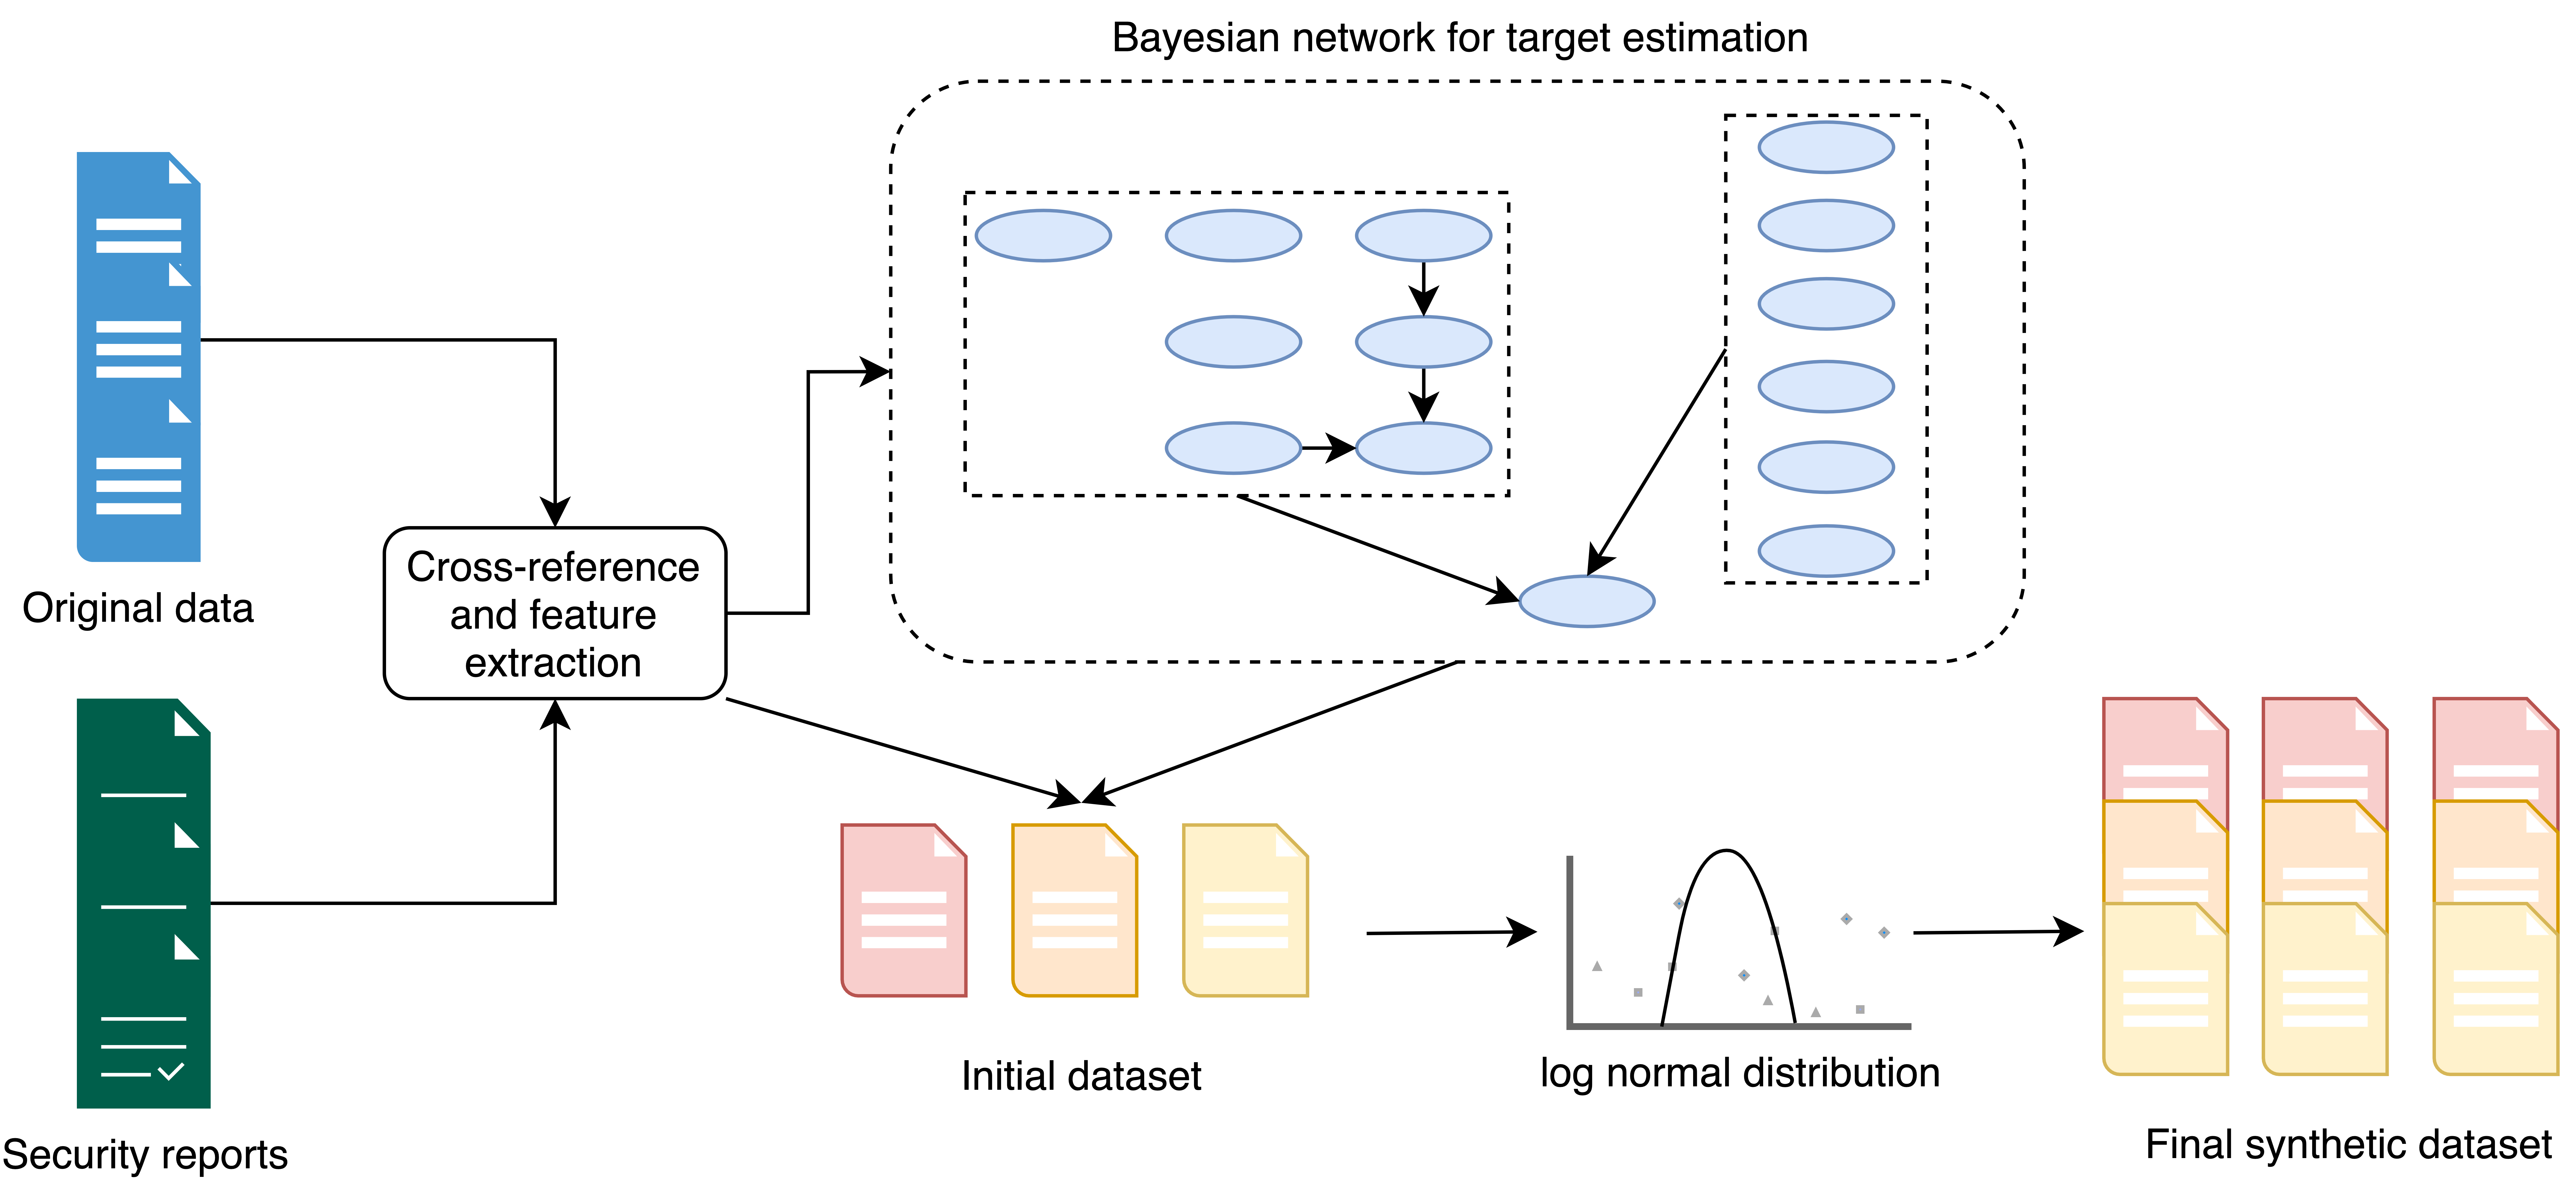
\includegraphics[scale=0.82]{images/synthetic/synthetic_data_complete}
	\caption{\label{fig:data_gen} Synthetic data generation process.}
\end{figure}

In a first part, we cross-reference the few questionnaires we were given with various security reports, and extract our dataset's features. This is presented in Section ~\ref{section:identify_feature}. In a second part, we build a Bayesian network based on the extracted features to estimate our dataset's targets. This is described in Section ~\ref{sec:target_estimation}. Finally, we use a log normal distribution to generate samples that share the same features but that have different target values. This is covered in Section ~\ref{section:generation}.  

\section{Features extraction}\label{section:identify_feature}

There are two components to any dataset: a set of features and a set of targets. The former describes attributes of the dataset's instances, while the latter captures the goal of the prediction task. The set of features and the set of targets should be closely related, otherwise the learning task becomes quite meaningless. Consider for instance the adult\footnote{\url{https://archive.ics.uci.edu/ml/datasets/adult}} dataset, where the prediction task is to determine whether or not a person makes over $50k$\$ a year. The set of features is composed of various attributes about the persons: their age, education, work-class, etc. These features are directly relevant to the prediction task, since they will influence the target value: a person that graduated high school versus a person that graduated from a Doctorate degree are likely to have a measurable income gap.


To identify our features, we need to understand how companies handle security, i.e. what are their security practices, and what are the implications on the \textit{loss} and \textit{cost} targets. These security practices can be technical (e.g. firewall configuration) or operational (e.g. does the company have a security and privacy policy that their employees must adhere to). Unfortunately, companies are likely to be concerned that honest answers indicating poor IT security practices could be used to discriminate against them. Hence, they are not very keen on releasing such information.

To shed some light on this, we went through annually released security reports from various vendors: Verizon \cite{verizon_report}, NetDiligence \cite{netdiligence_report}, IBM \cite{ibm_report}, Cisco \cite{cisco_report}, Checkpoint \cite{checkpoint_report}, and AIG \cite{aig_report}. These reports highlight current security practices that company follow (or, fail to follow) and provide insights about the threat landscape they face, in an anonymised fashion. Of particular relevance to our business problem, the NetDiligence \cite{netdiligence_report} and AIG \cite{aig_report} reports provide data from the insurer's perspective, highlighting common causes and consequences about cyber attacks that their clients suffered.

Using these reports, we can derive useful probabilities. NetDiligence \cite{netdiligence_report} shows that in the $2014-2018$ period, social engineering (act of tricking someone into divulging information or taking action) was responsible for 28\% of the claims they received from companies. Since this number is post-incident, we can transform it into a conditional probability between the event \textit{social engineering} and the event \textit{the company suffers a loss}: $Pr(social\_engineering | loss) = 0.28$. To benefit our synthetic data generation problem, we can tweak this a little and create a new feature, \textit{$f_1$ = company\_trains\_employees\_against\_social\_engineering}. We can now artificially derive: $Pr(f_1 | loss) = 1 - Pr(social\_engineering | loss) = 1 - 0.28 = 0.72$. It could be argued that for some companies, training was delivered but improperly, thus raising questions about the probability that was derived. For this thesis and for the sake of simplicity, we will assume an ideal scenario.

Following a similar approach, we derive multiple such features and probabilities across all the reports, which we summarise in Table ~\ref{table:probs}. If multiple vendors report about the same incident (e.g. social engineering), we take the mean value that was reported across all reports. As these reports do not provide pre-incident figures (e.g., $Pr(f_1)$), we manually assign a probability to such events, where relevant. We additionally create the following features for which the reports did not provide any information: \textit{company\_uses\_3rd\_party}, \textit{company\_has\_ids\_ips}, \textit{company\_has\_recovery\_plan}, \textit{company\_has\_firewalls}. For the company sector, we create a single feature \textit{sector} which can be one of $[hospitality, \; manufacturing, \; energy, \; \dots]$. We let the reader refer to Table ~\ref{table:features_meaning} for more information about the features and their meaning.

While the companies' security practices will likely influence the \textit{loss} target, not all features influence the \textit{cost} target. Typically, \textit{$f_1$ = social\_engineering} is not expected to contribute to the \textit{cost} target, as this target is post-incident: employees being trained against social engineering is not expected to influence how much the company will lose once an incident has happened. To make up the \textit{cost} target, we need to position ourselves on the attacker's side. Once an initial foothold inside the company has been established, the kind of data they may be able to find is likely to be relevant, as it will allow them to progress their attack further.

The Verizon report \cite{verizon_report} gives us a breakdown of the type of data that each industry is likely to possess: PII (personal identifiable information), PCI (payment card industry), PHI (protected health information), credentials (passwords), or 'other'. This is reported in Table ~\ref{table:probs-data}. This allows us to derive further features: \textit{company\_has\_pii, company\_has\_pci, company\_has\_phi, etc}.

\begin{center}\begin{table}[h!]
	\center
	\noindent\makebox[0pt]{}{
		\begin{tabular}{|c|c|c|c|c| } 
 		\hline
 		Feature ($F$) & $Pr(F)$ & $Pr(F | loss)$ & $Pr(F|SME)$ & $Pr(F| large)$ \\ [0.5ex] \hline\hline
 		$company\_is\_in\_hospitality$ & & & 0.03 & 0.04 \\ \hline
 		$company\_is\_a\_public\_entity$ & & & 0.03 & \\ \hline
 		$company\_is\_in\_other$ & & & 0.11 & 0.09 \\ \hline
 		$company\_is\_a\_nonprofit$ & & & 0.05 & \\ \hline
 		$company\_is\_in\_education$ & & & 0.05 & 0.08 \\ \hline
 		$company\_is\_in\_technology$ & & & 0.06 & 0.03\\ \hline
 		$company\_is\_in\_manufacturing$ & & & 0.08 & 0.03 \\ \hline
 		$company\_is\_in\_financial\_services$ & & & 0.09 & 0.15\\ \hline
 		$company\_is\_in\_energy$ & & & & 0.04 \\ \hline
 		$company\_is\_in\_retail$ & & & 0.09 & 0.24\\ \hline
 		$company\_is\_in\_healthcare$ & & & 0.19 & 0.26\\ \hline
 		$company\_is\_in\_professional\_services$ & & & 0.22 & 0.04 \\ \hline
 		\makecell{$company\_trains\_employees\_$\\$against\_social\_engineering$} & 0.70 & 0.8025 & & \\ \hline
 		$company\_has\_patching\_process$ & 0.60 & 0.828 & & \\ \hline
 		$company\_has\_antivirus$ & 0.95 & 0.81 & & \\ \hline
 		$company\_uses\_3rd\_party$ & 0.87 & & & \\ \hline
 		$company\_has\_ids\_ips$ & 0.94 & & & \\ \hline
 		$company\_has\_recovery\_plan$ & 0.33 & & & \\ \hline
 		$company\_has\_firewalls$ & 0.83 & & & \\ \hline
	\end{tabular}
	\caption{\label{table:probs} Potential features for the synthetic dataset and their respective probabilities. We separate small and medium sized businesses (SME) from large businesses.}}
\end{table}\end{center}

\begin{center}\begin{table}[h!]
	\center
	\noindent\makebox[0pt]{}{
		\begin{tabular}{|c|c|c|c|c|c|} 
 		\hline
 		Sector ($S$) & $Pr(PII | S)$ & $Pr(PCI|S)$ & $Pr(PHI|S)$ & $Pr(credentials|S)$ & $Pr(other|S)$ \\ [0.5ex] \hline\hline
 		$Hospitality$ & 0.44 & & & 0.34 & 0.23 \\ \hline
 		$Public \; Entity$ & 0.51 & & & 0.33 & 0.34\\ \hline
 		$Other$ & 0.81 & & & 0.36 & 0.42 \\ \hline
 		$Education$ & 0.75 & & & 0.30 & 0.23 \\ \hline
 		$Technology$ & 0.69 & & & 0.41 & 0.34 \\ \hline
 		$Manufacturing$ & 0.49 & 0.20 & & 0.55 & 0.25 \\ \hline
 		$Financial \; Services$ & 0.77 & 0.32 & & 0.35 & 0.35 \\ \hline
 		$Energy$ & 0.41 & 0.68 & & 0.41 & 0.35 \\ \hline
 		$Retail$ & 0.49 & 0.47 & & 0.27 & 0.25 \\ \hline
 		$Healthcare$ & 0.77 & & 0.67 & 0.18 & 0.18 \\ \hline
 		$Professional \; Services$ & 0.75 & & & 0.45 & 0.32 \\ \hline
	\end{tabular}
	\caption{\label{table:probs-data} Probabilities for companies within a specific sector to store a certain type of data}}
\end{table}\end{center}

\section{Targets estimation}\label{sec:target_estimation}

Section ~\ref{section:identify_feature} introduced a way to identify the set of features for our synthetic dataset, and their corresponding probabilities for feature selection. Feature selection consists in deciding if a feature is \textit{True} or \textit{False} for a given company. For instance, the social engineering feature $f_1$ has a probability of $Pr(f_1) = 0.70$ according to Table ~\ref{table:probs}. During the data generation process, each instance will see this feature set to \textit{True} with probability 0.70, and to \textit{False} with probability 0.30. This process of feature selection is repeated across all features. Once this is done, we must use the results of the feature selection process to compute fictive values for our targets \textit{loss} and \textit{cost}. This section presents two approaches, both using Bayesian networks, that vary in complexity.


\begin{definition}[Graphical model \cite{bayes}]
	A graphical model is a tool that is used to visually illustrate and work with conditional independencies among variables in a given problem.
\end{definition}

A graph is composed of a set of nodes (which represent the variables) and a set of edges. Each edge connects two nodes, and an edge can have an optional direction associated to it. Two variables are conditionally independent if they have no direct impact on each other's value. Figure ~\ref{fig:graph_model} shows an example of a graphical model.

\begin{figure}[h!]
	\center
	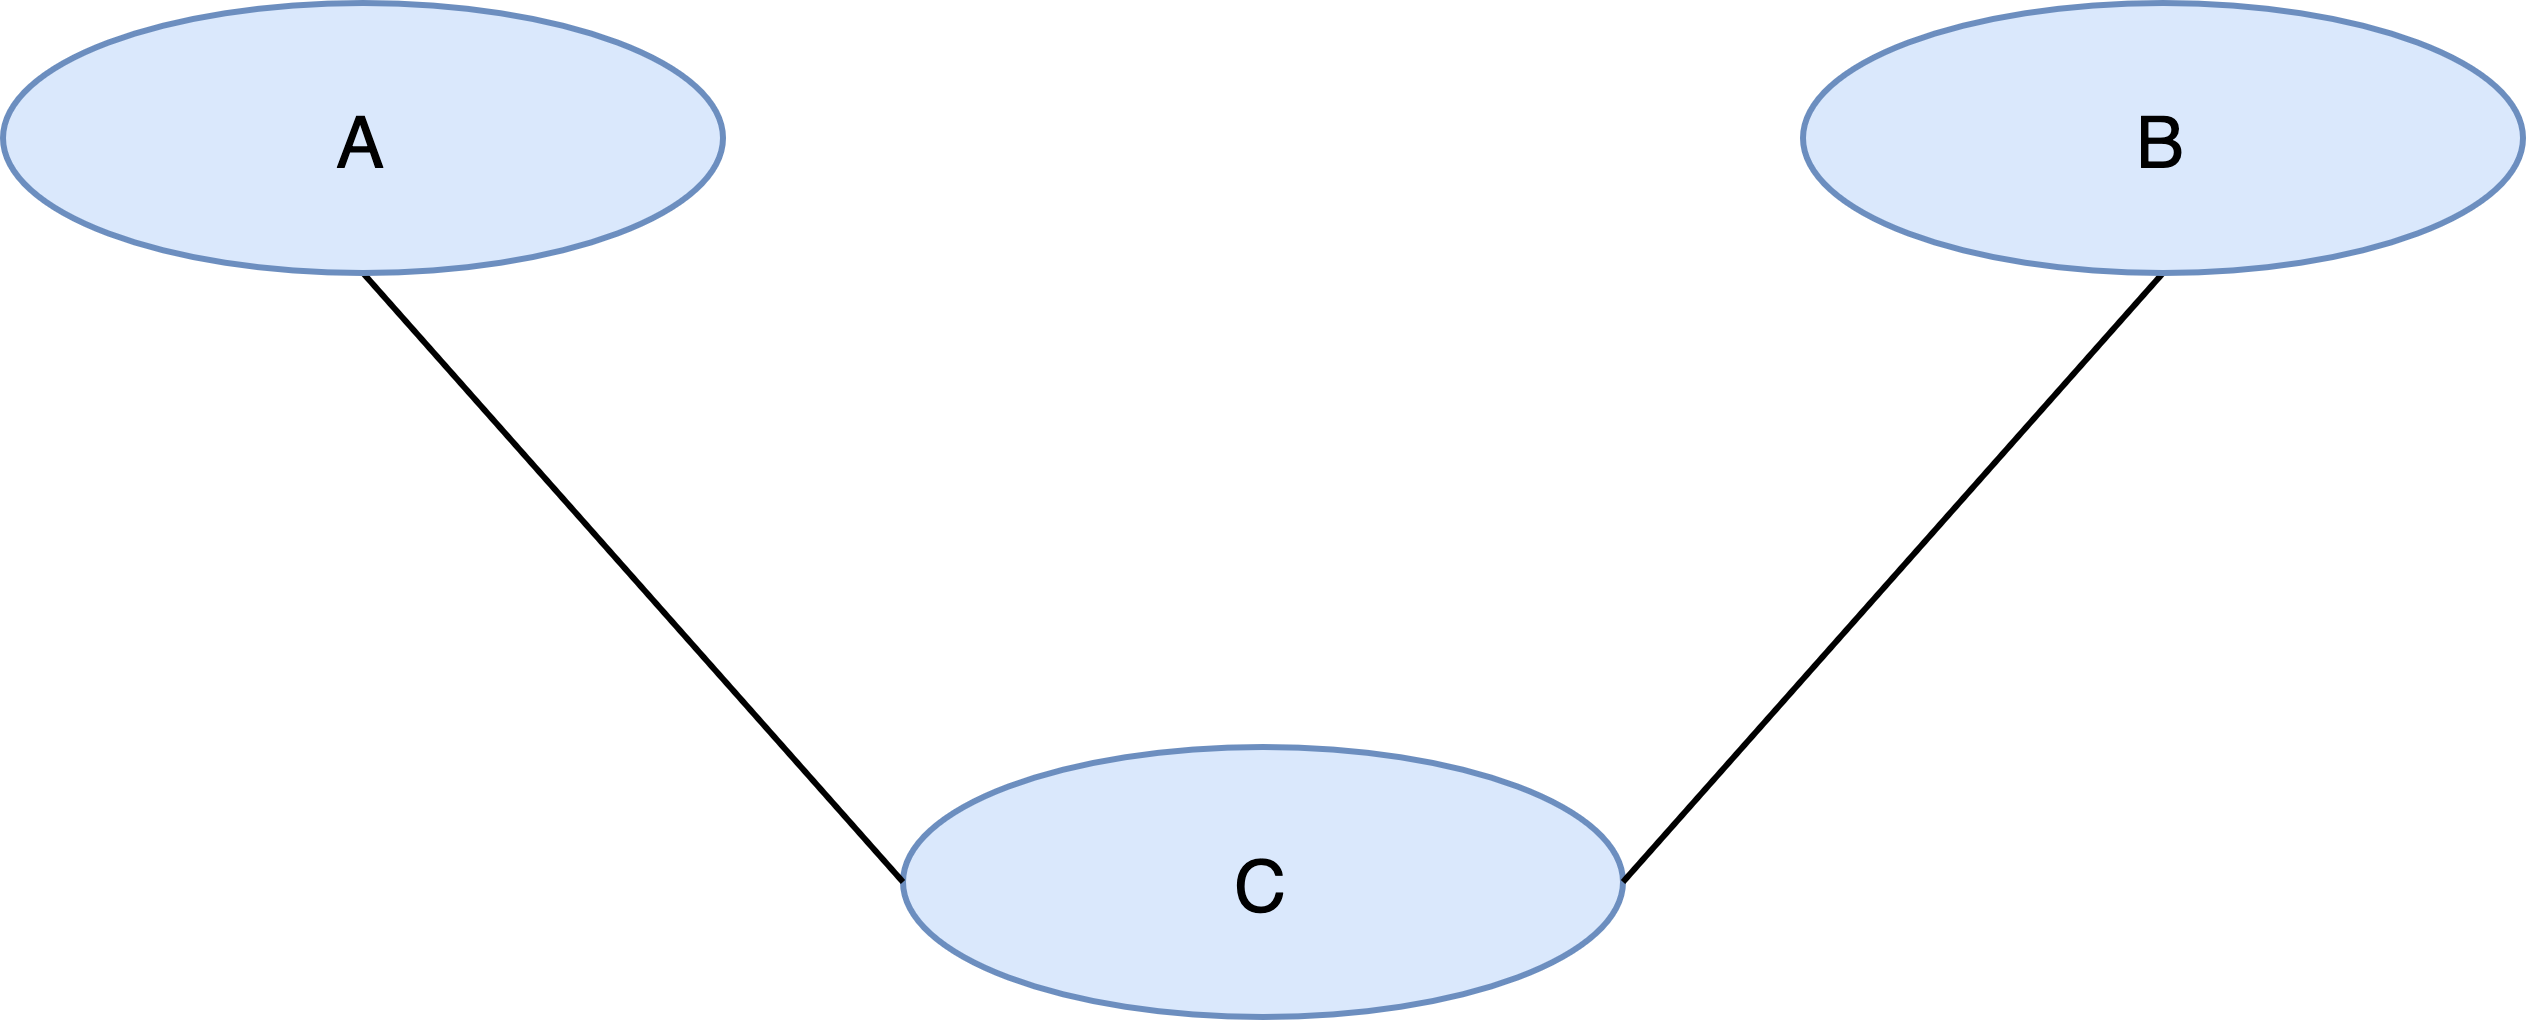
\includegraphics[scale=0.63]{images/synthetic/graphical_model.png}
	\caption{\label{fig:graph_model} A graphical mode,  in which A and B are conditionally independent given C.}
\end{figure}

\begin{definition}[Bayesian network \cite{bayes}]
	Bayesian networks are a particular instance of graphical models. They are directed acyclic graphs (DAG): all edges in the graph are directed (i.e. they point in a particular direction) and there are no cycles (i.e. there is no way to start from a node, travel along a set of directed edges and arrive back at the starting node).
\end{definition}

Figure ~\ref{fig:bayesian} illustrates a Bayesian network. Given nodes $\textbf{X} = X_1, \dots, X_n$, the joint probability function for any Bayesian network is $Pr(\textbf{X}) = \prod_{i=1}^nPr(X_i | parents(X_i))$. This means that the joint probability of all the variables is the product of the probabilities of each variable given its parents' value. In Figure ~\ref{fig:bayesian}, we have $Pr(A,B,C) = Pr(A)Pr(B)Pr(C|A,B)$.

\begin{figure}[h!]
	\center
	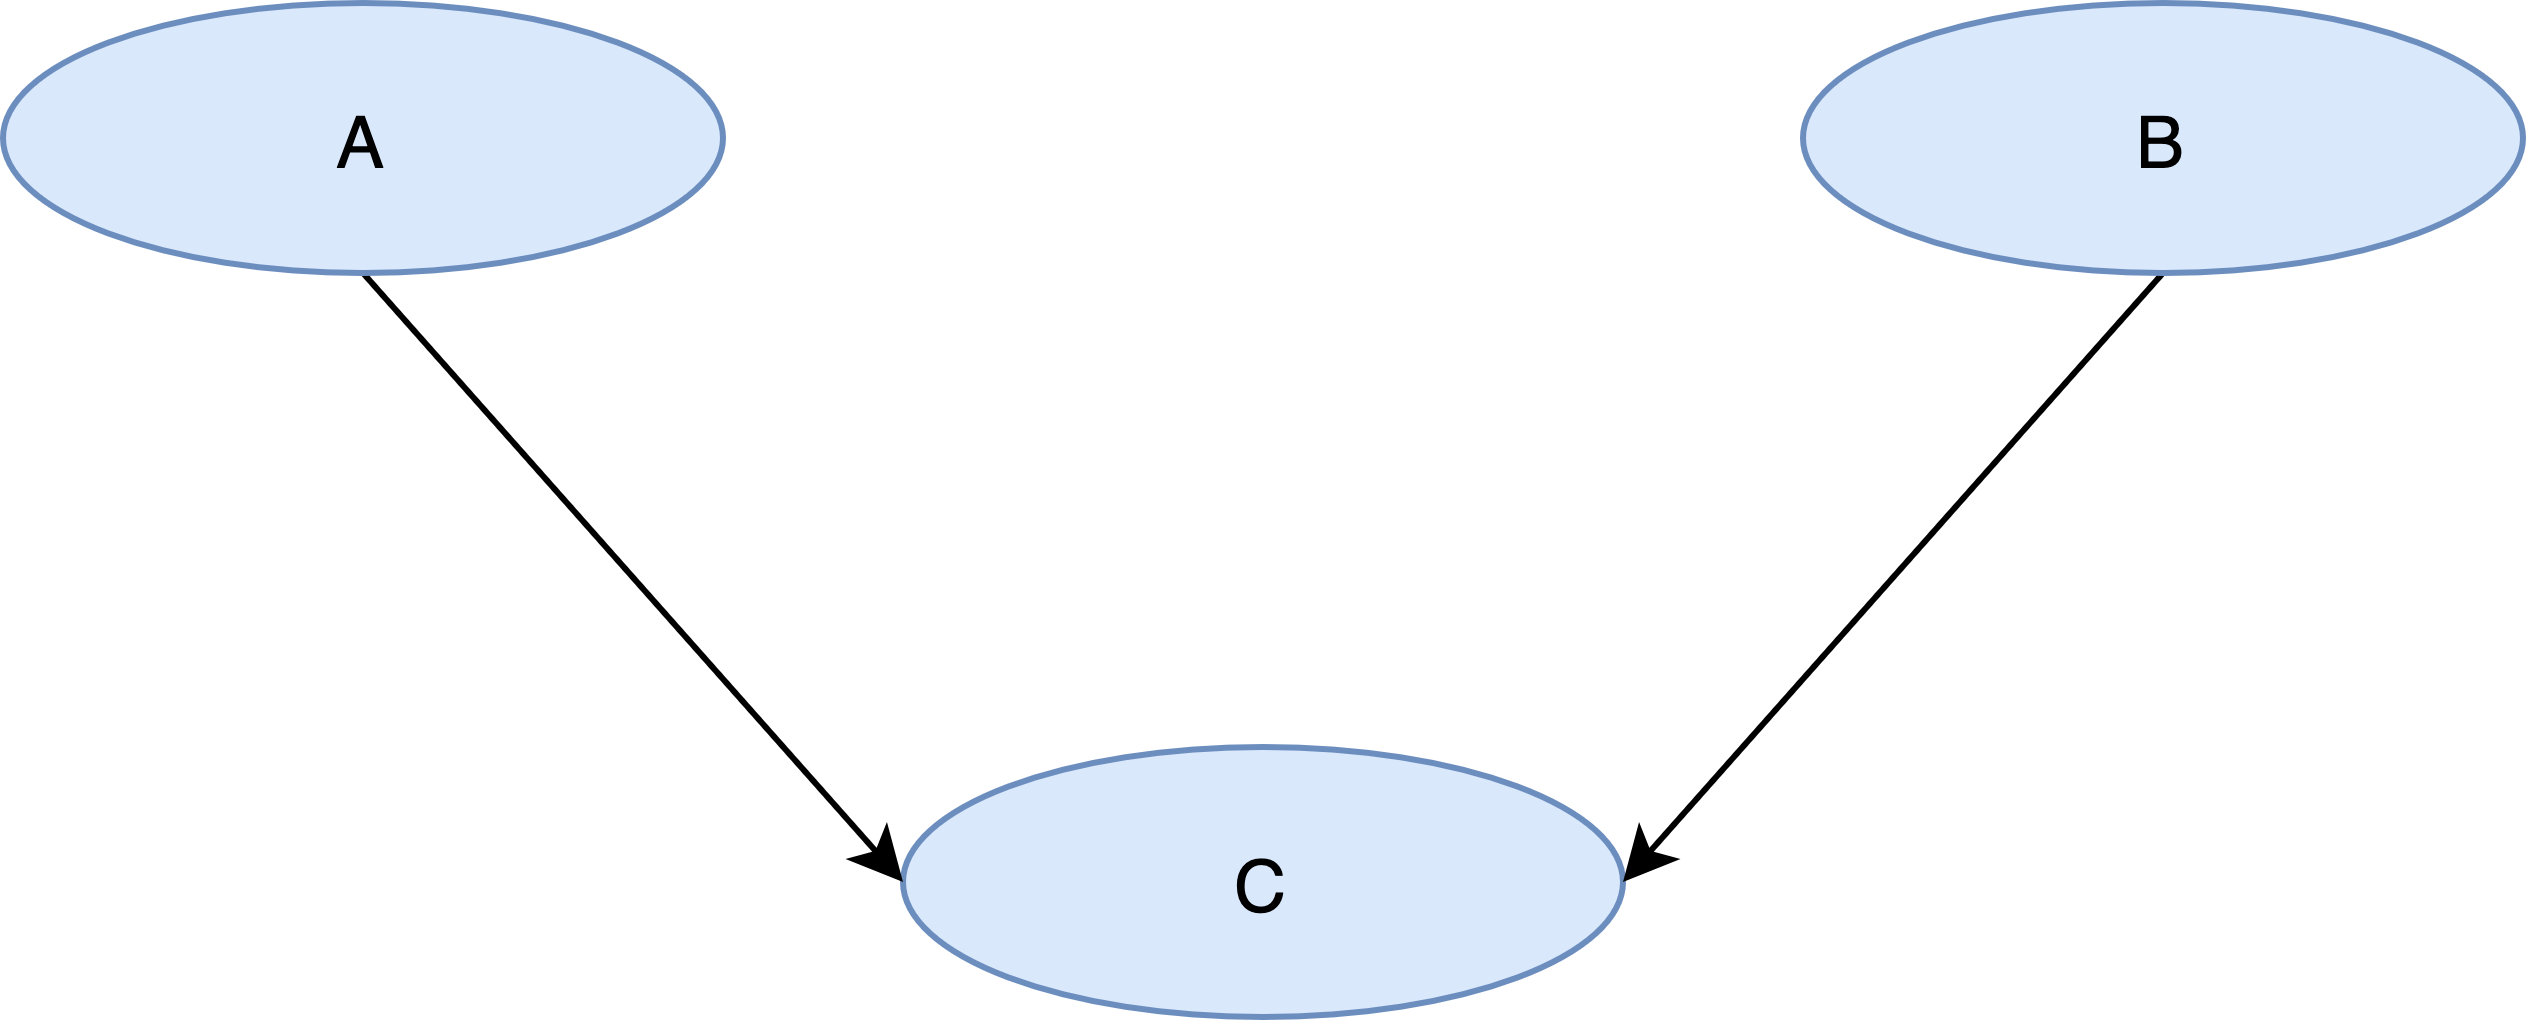
\includegraphics[scale=0.63]{images/synthetic/bayesian.png}
	\caption{\label{fig:bayesian} A simple Bayesian network.}
\end{figure}

\subsection{Approach 1}

\subsubsection{Loss target}

For the \textit{loss} target, we propose the Bayesian network outlined in Figure ~\ref{fig:bayesian-easy}. We make the \textit{loss} target depend on a subset of the features: \textit{social engineering training}, \textit{antivirus}, and \textit{outdated software patching process}. Since the reports do not mention any correlations between these features, we assume that they are conditionally independent with respect to \textit{loss}.

\begin{figure}[h!]
	\center
	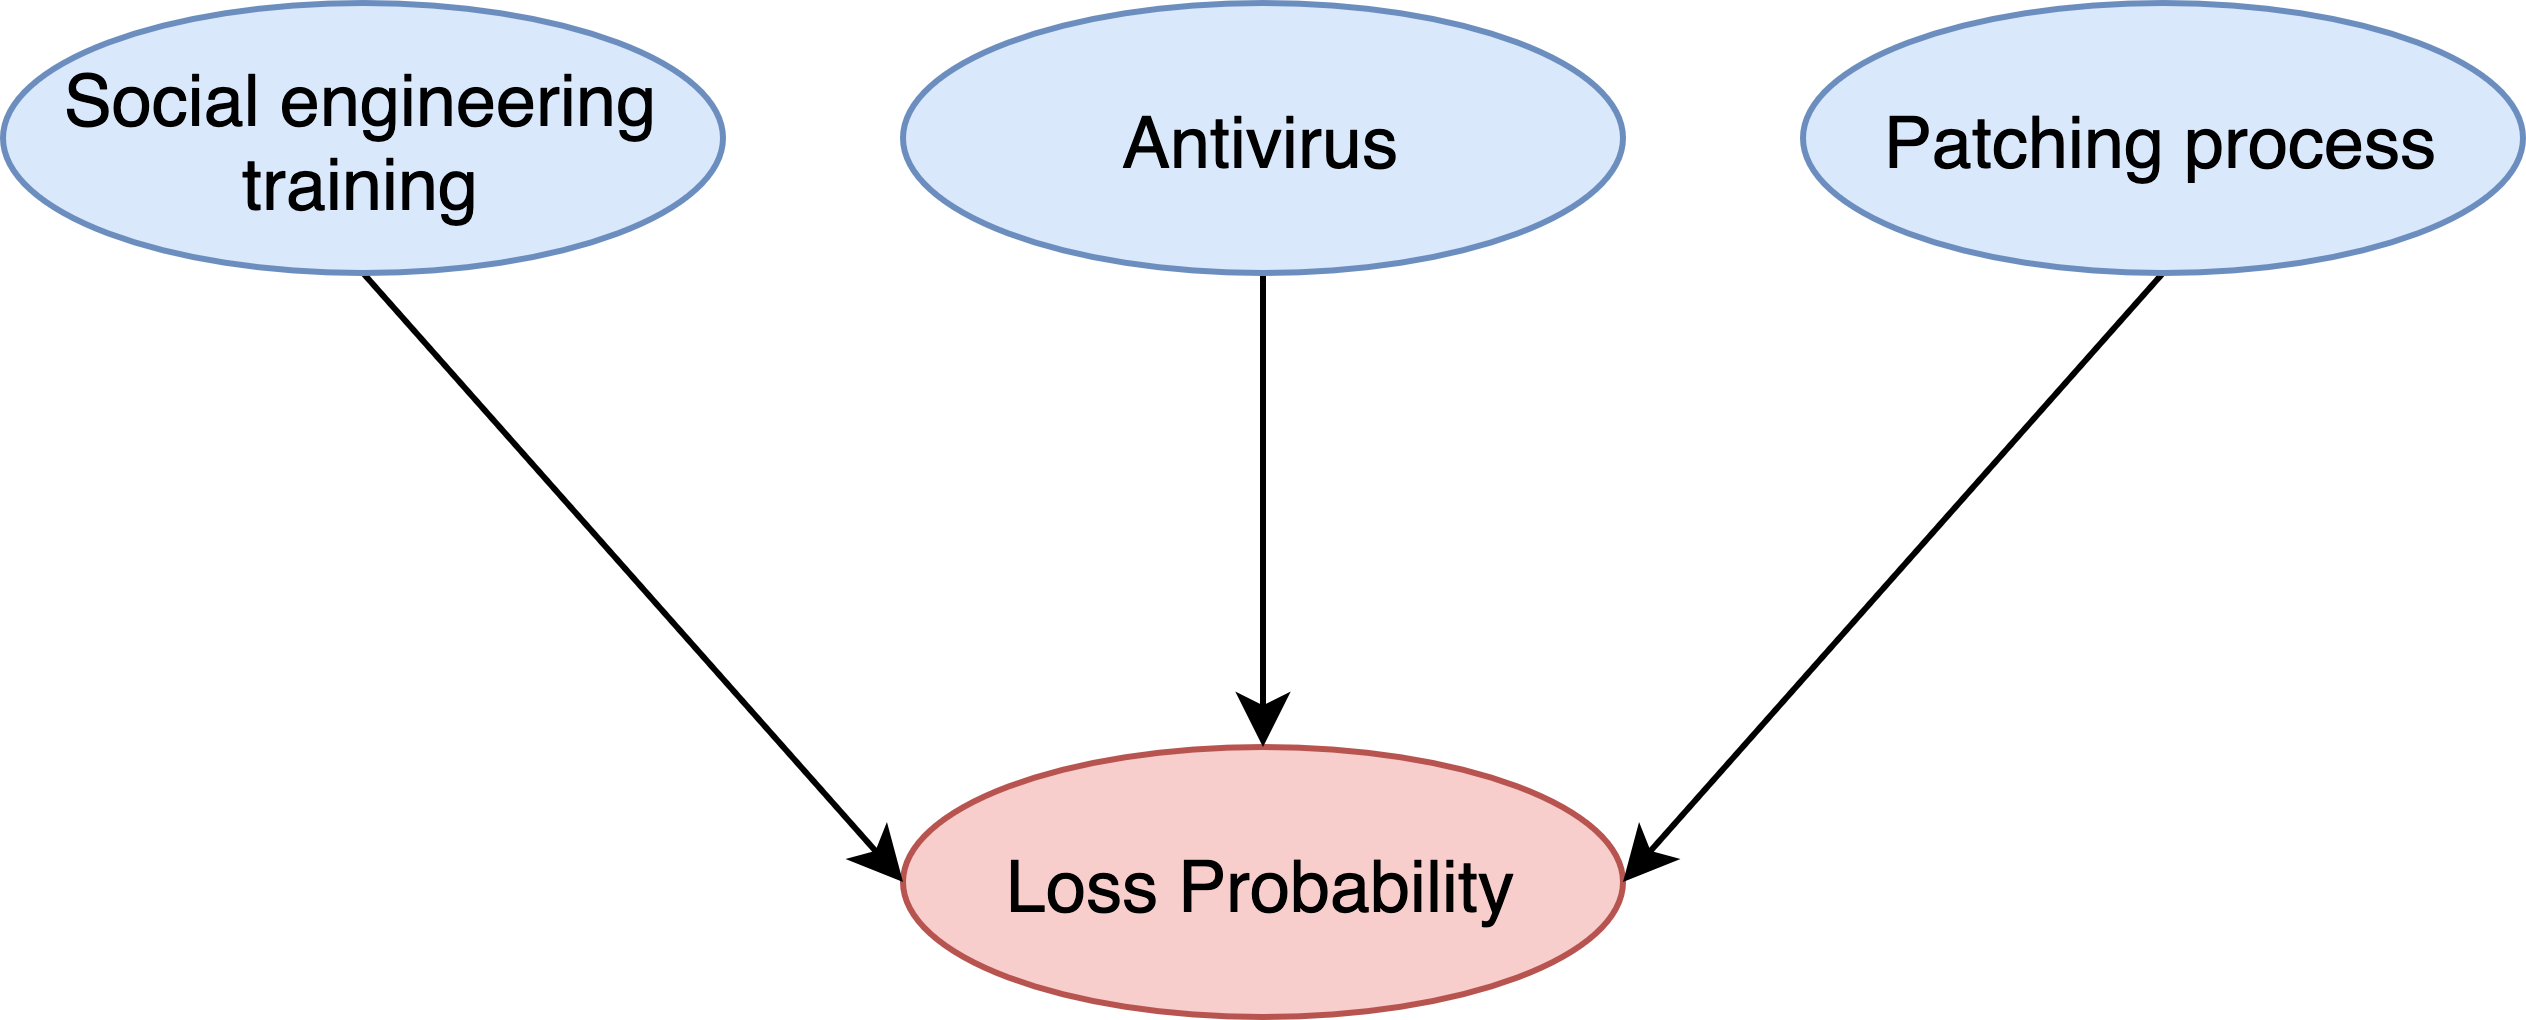
\includegraphics[scale=0.63]{images/synthetic/bayesian_easy}
	\caption{\label{fig:bayesian-easy} Bayesian network for the \textit{loss} target.}
\end{figure}

We can then derive: 

\begin{equation} \label{eq1}
\begin{split}
Pr(loss | social, antivirus, patching) & = \frac{Pr(loss, social, antivirus, patching)}{Pr(social)Pr(antivirus)Pr(patching)} \\
 & = \frac{Pr(social, antivirus, patching | loss)Pr(loss)}{Pr(social)Pr(antivirus)Pr(patching)} \\
 & = \frac{Pr(social|loss)Pr(antivirus|loss)Pr(patching|loss)}{Pr(social)Pr(antivirus)Pr(patching)}
\end{split}
\end{equation}

Fixing $Pr(loss) = 0.10$ and plugging in the data provided in Table ~\ref{table:probs}, we can compute the \textit{loss} target.

\subsubsection{Cost target}

To derive a number for the target \textit{cost}, we exclusively rely on data provided in the NetDiligence \cite{netdiligence_report} report:

\begin{itemize}
	\item The \texttt{min}, \texttt{max} and \texttt{mean} cost of a breach in a particular industry: $min(cost_{breach})$, $max(cost_{breach})$, $mean(cost_{breach})$
	\item The \texttt{mean} post-incident (crisis) cost, i.e. the breach remediation cost $cost_{remediation}$
	\item The \texttt{mean} cost per type of data that was potentially exposed, $cost_{data}$. This cost directly depends on the features of a given instance: if the instance is in healthcare, then as per Table ~\ref{table:probs-data}, we will add together the costs for leaked PII, PHI, credentials and others if these attributes are \textit{True} for that instance.
\end{itemize}

In particular, we derive the cost as per the following formula: $cost = triangular(min(cost_{breach}),$ $max(cost_{breach}), mean(cost_{breach})) + cost_{remediation} + \sum_{data}{cost_{data}}$ where $triangular()$ is the triangular distribution. Fig. ~\ref{fig:distribution-easy} shows the distribution of values for the targets over 1 million generated samples. The method used to generate the samples is detailed in Section ~\ref{section:generation}.

\begin{figure}[h!]
	\center
	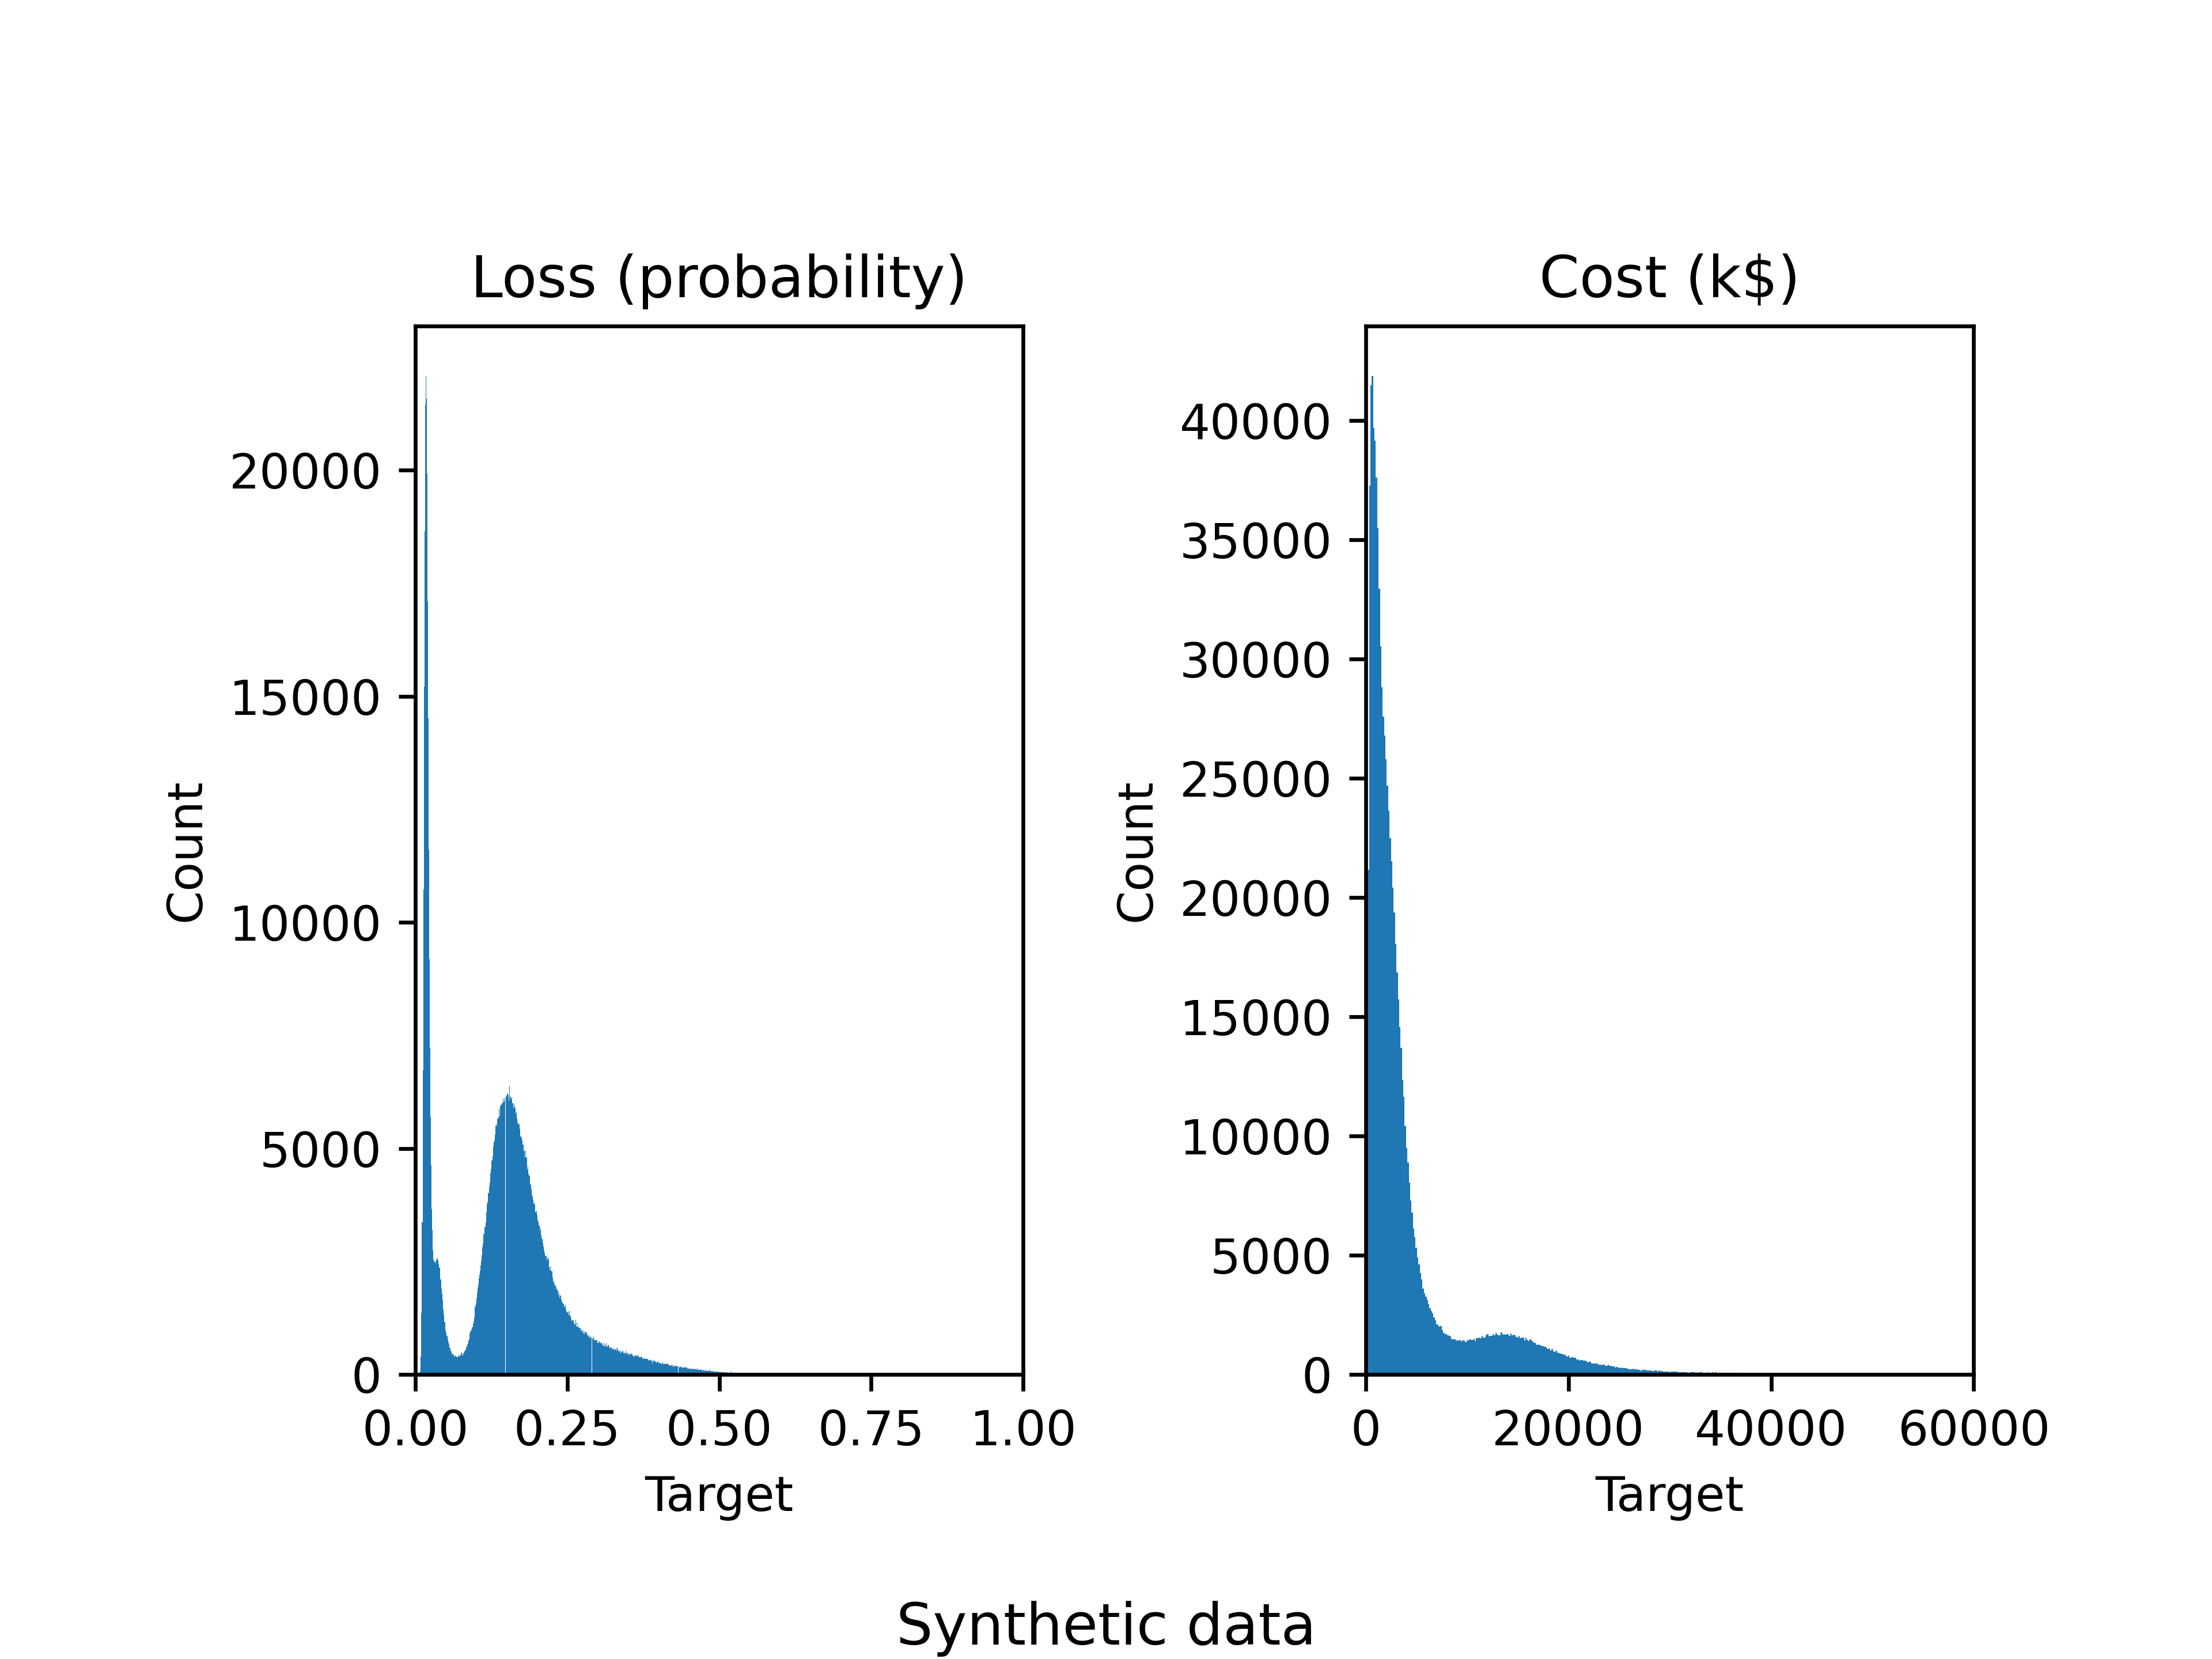
\includegraphics[scale=0.51]{images/synthetic/easy_distribution.png}
	\caption{\label{fig:distribution-easy} Target distribution for the synthetic dataset.}
\end{figure}

Unfortunately, our testing demonstrated that the problem was rendered hard through too much randomness / noise addition, rather than by the intricacies of the features and the targets themselves. This is why we now propose a second approach to the problem.

\subsection{Approach 2}

\subsubsection{Loss target}\label{subsubsection:prob_loss}

For the \textit{loss} target, we propose a more complex Bayesian network, as depicted in Figure ~\ref{fig:bayesian-hard}. Table ~\ref{table:all_probs} summarises the probabilities that we used in this model. Following the logic of Equation ~\ref{eq1}, we can derive:

\begin{figure}[h!]
	\center
	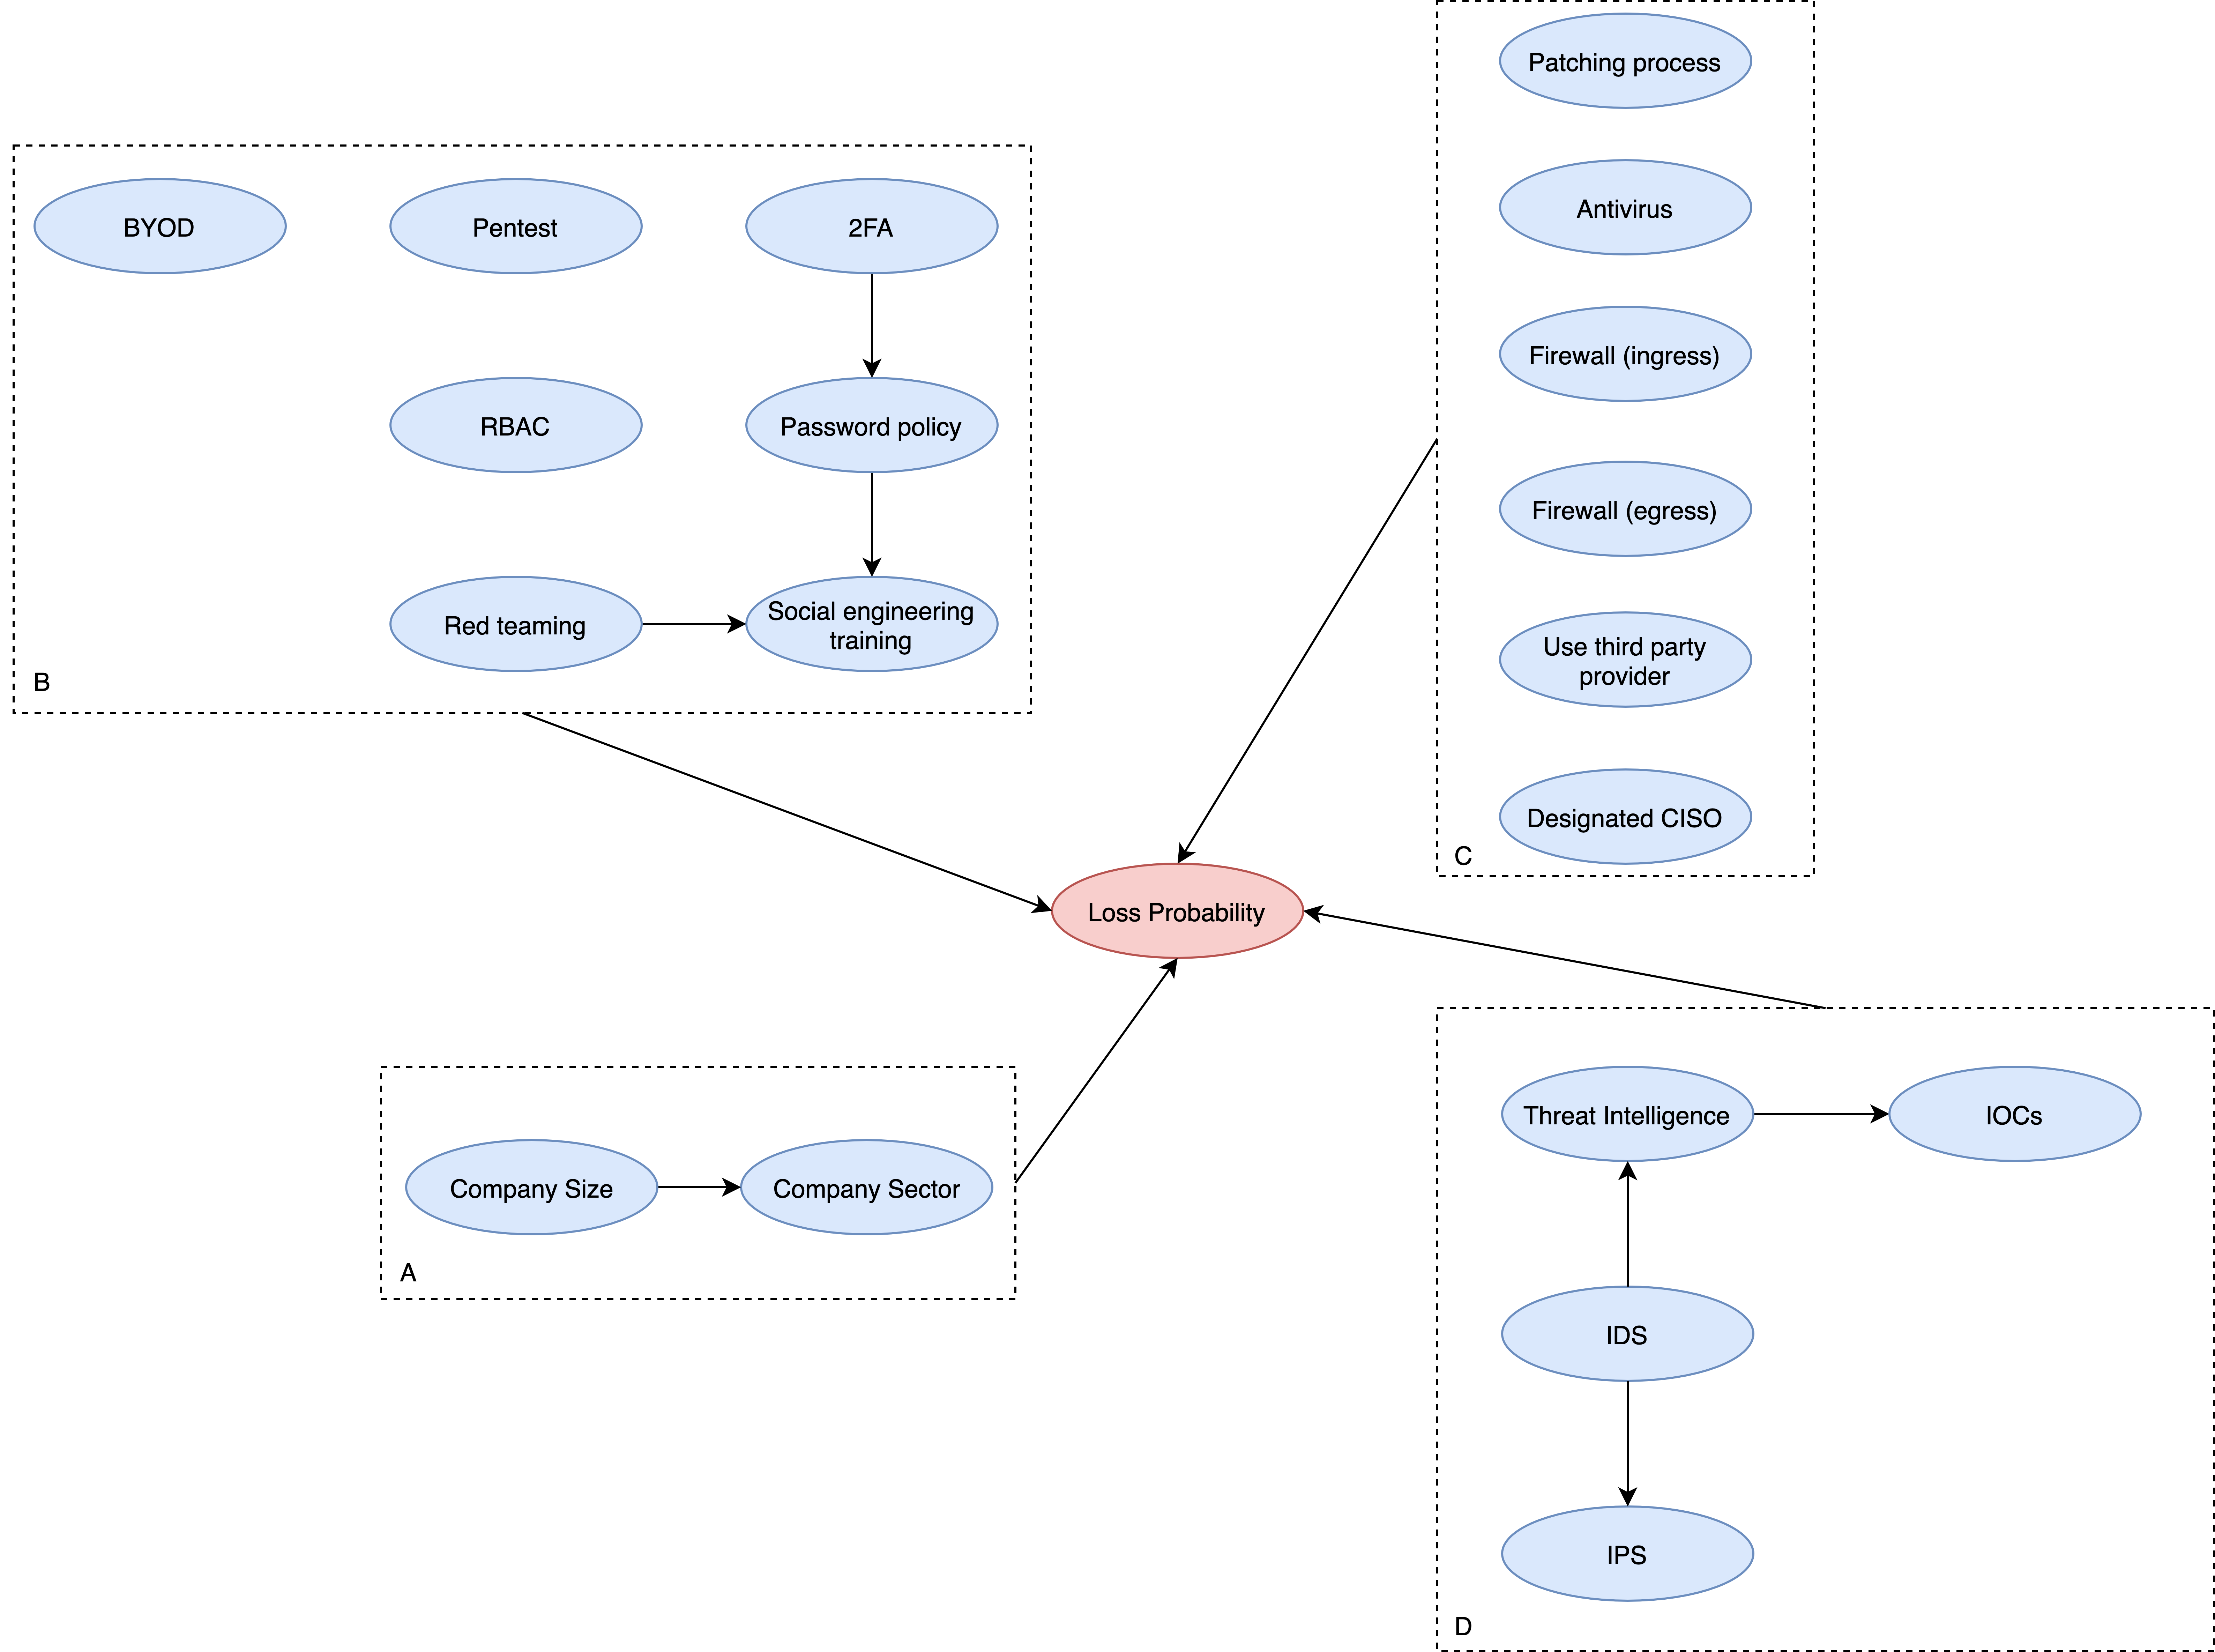
\includegraphics[scale=0.60]{images/synthetic/bayesian_hard.png}
	\caption{\label{fig:bayesian-hard} Revisited Bayesian network for the \textit{loss} target.}
\end{figure}

\begin{equation} \label{eq2}
\begin{aligned}
\begin{split}
Pr(A) & = Pr(company\_size | company\_sector)Pr(company\_size) \\
Pr(A|loss) & = Pr(company\_size, company\_sector | loss) \\
Pr(B) & = {Pr(BYOD)Pr(pentest)Pr(RBAC)Pr(red\_teaming)Pr(2FA)Pr(pwd\_policy | 2FA)}\\ 
& \ \ \ \ Pr(social|pwd\_policy,red\_teaming) \\
Pr(B|loss) & = Pr(BYOD|loss)Pr(pentest|loss)\\
& \ \ \ \ \ Pr(RBAC|loss)Pr(red\_teaming, 2FA, pwd\_policy,soc|loss) \\
Pr(C) & = Pr(patching)Pr(antivirus)Pr(fw\_ingress)Pr(fw\_egress)Pr(3rd\_party)Pr(CISO)\\
Pr(C|loss) & = Pr(patching|loss)Pr(antivirus|loss)Pr(fw\_ingress|loss)Pr(fw\_egress|loss) \\
& \ \ \ \ \ Pr(3rd\_party|loss)Pr(CISO|loss) \\
Pr(D) & = Pr(IPS|IDS)Pr(IDS)Pr(threat|IDS)Pr(IOC|threat) \\
Pr(D|loss) & = Pr(IPS, IDS, threat, IOC|loss)
\end{split}
\end{aligned}
\end{equation}

Which we can plug into:

\begin{equation} \label{eq6}
\begin{split}
Pr(loss|A,B,C,D) = \frac{Pr(A|loss)Pr(B|loss)Pr(C|loss)Pr(D|loss)Pr(loss)}{Pr(A)Pr(B)Pr(C)Pr(D)}
\end{split}
\end{equation}

\subsubsection{Cost target}\label{subsubsection:cost_calc}

For the \textit{cost} target, we propose additional features that influence the outcome, as shown in Figure ~\ref{fig:cost}. The cost is now computed as:

\begin{equation}\label{eq7}
	cost = \sum_{data}{cost_{data}} + \lambda_1mean(cost_{breach}) + \lambda_2cost_{remediation}
\end{equation}
where $\lambda_1$ and $\lambda_2$ $\in [0, 1]$ represent the fraction of the cost that should be applied to the instance. They are computed at runtime depending on the instance's features. For example, if the instance has the feature \textit{company\_has\_incident\_response\_team} set to \textit{True}, then we decrease $\lambda_2$ by a certain amount, as we expect the remediation cost to be lower in the presence of an IR team.

\begin{figure}[h!]
	\center
	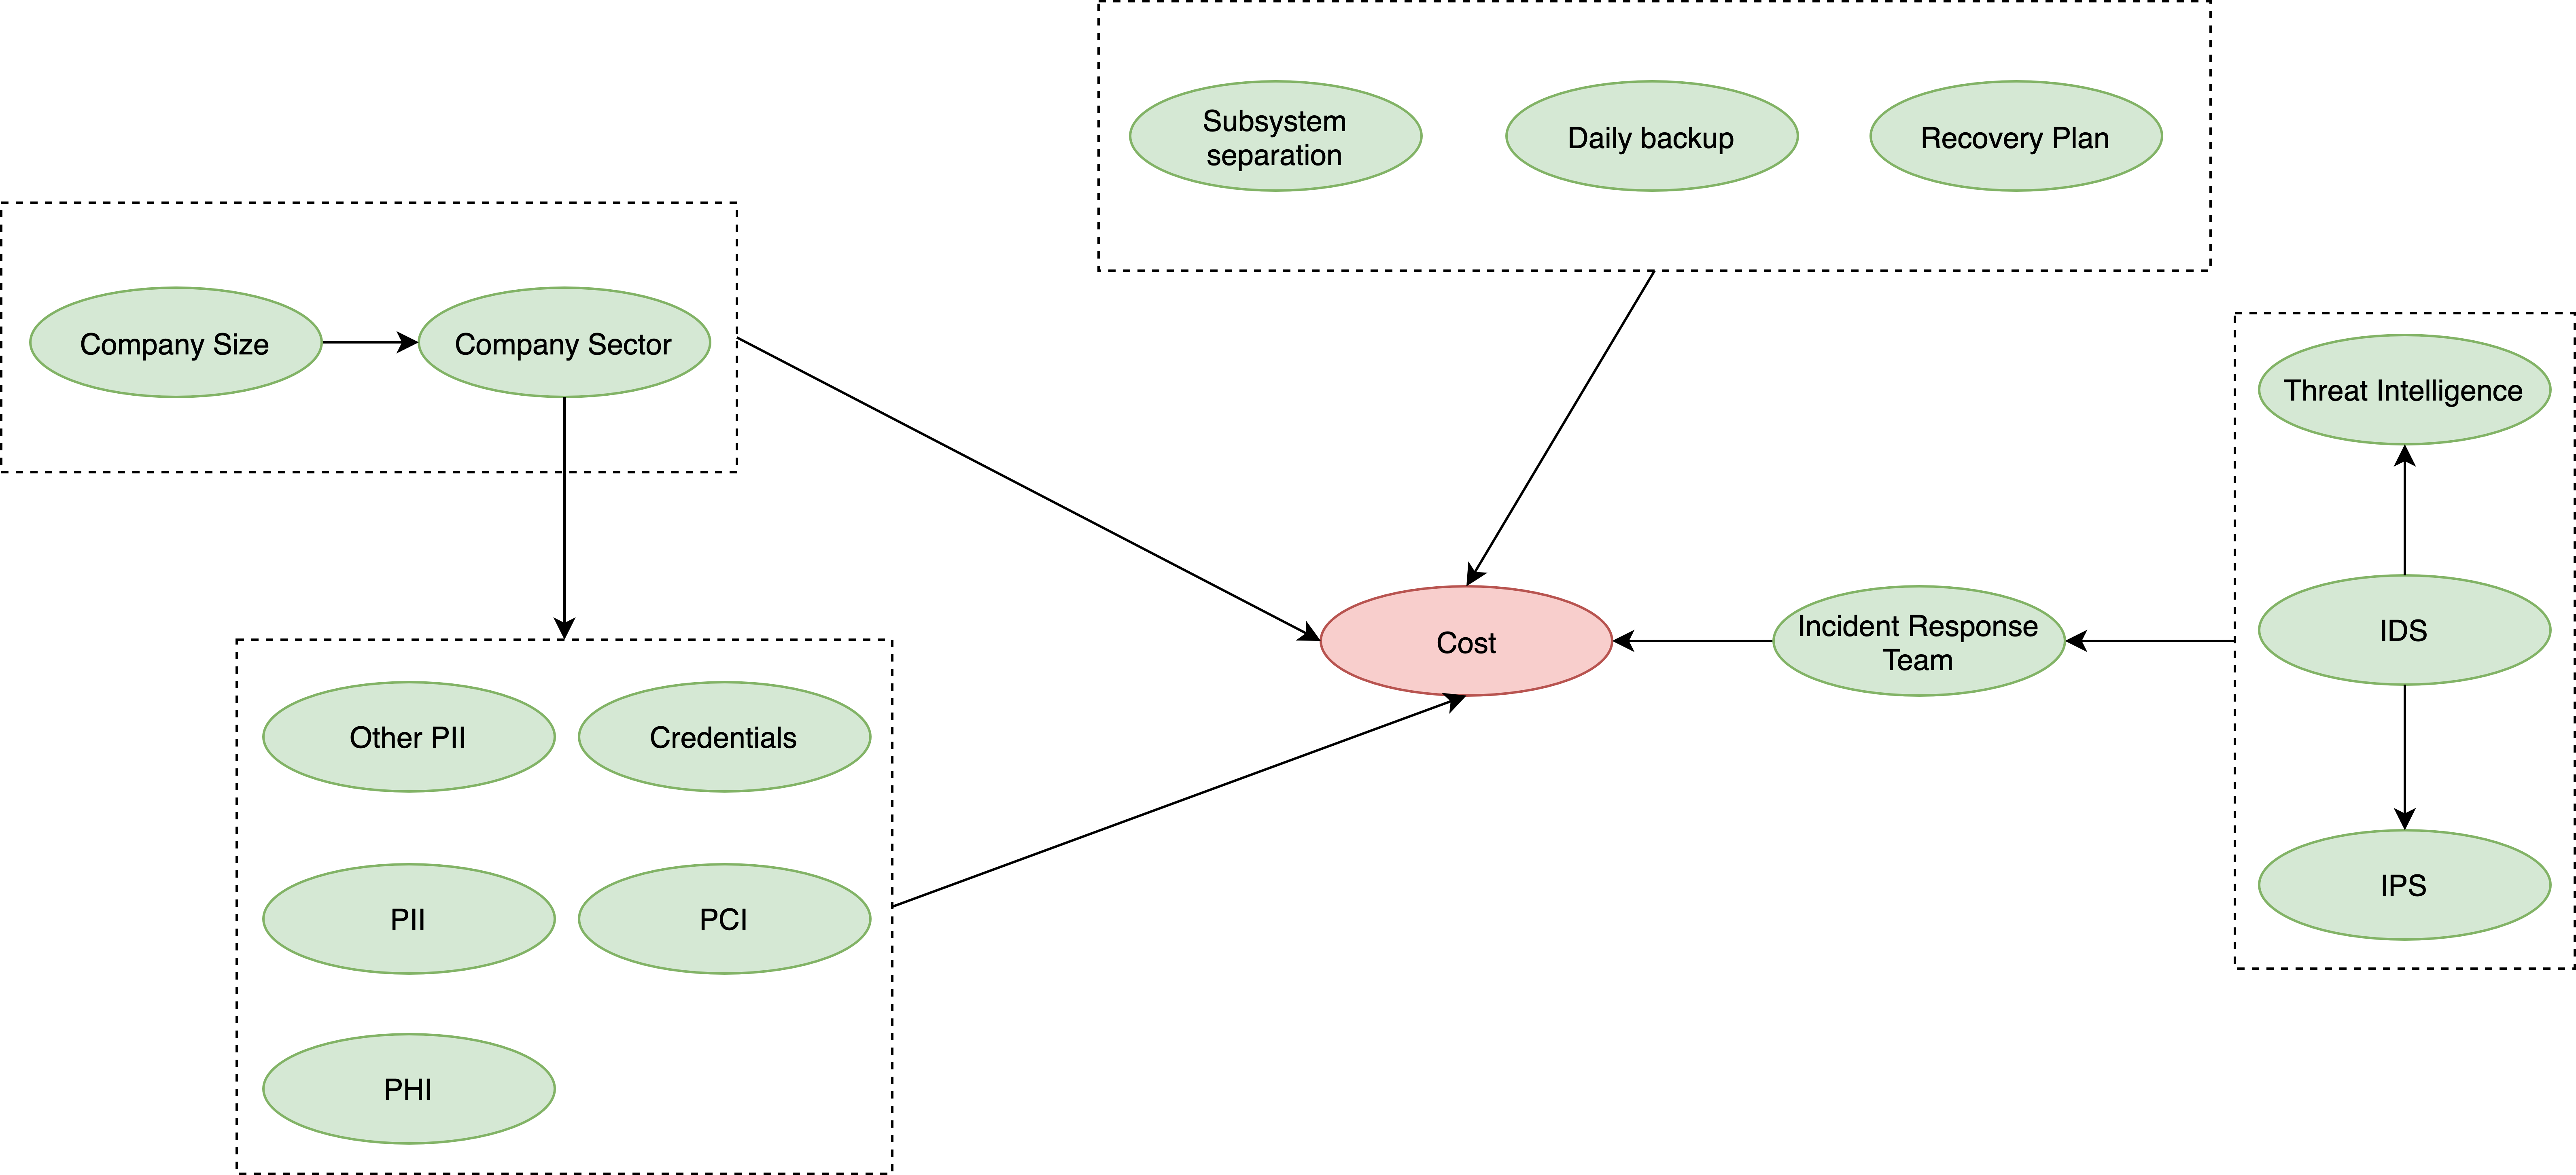
\includegraphics[scale=0.6]{images/synthetic/cost.png}
	\caption{\label{fig:cost} Features that influence the \textit{cost} target.}
\end{figure}

We generate 4 synthetic datasets, each of 1 million samples, using this new approach. The distributions of the targets are depicted in Figure ~\ref{fig:distribution-hard}.

\section{Data generation}\label{section:generation}

We start the data generation process by first creating what we called an \textit{instance stereotype}. An instance stereotype is an instance with a defined set of features (e.g. $company\_has\_antivirus: True, \; company\_has\_IDS: True, \; company\_has\_IPS: False, \; \dots$).  In practice, we expect that instances may share the same features while having slightly different target values. This is because there are many other factors that influence the \textit{loss} and \textit{cost} targets in real life, which are not captured here. For instance, two companies may both have an incident response team but their process may differ, and incident containment could take  the first company two hours and the second one two days, which may in turn impact the \textit{cost} target.  To model these differences, we rely on a log normal distribution.

\begin{definition}[Log normal distribution]
Let $Z$ be a standard normal variable, and let $\mu$ and $\sigma > 0$ be two real numbers. Then, the distribution of the random variable $X=e^{\mu+\sigma Z}$ is called the log-normal distribution with parameters $\mu$ and $\sigma$. \\

\textbf{Note}: $\mu$ and $\sigma$ are the parameters of the variable's natural logarithm, not of $X$ itself. In order to produce a distribution with desired mean $\mu_X$ and standard deviation $\sigma_X$, one uses $\mu=\ln\left(\frac{\mu_X^2}{\sqrt{\left(\mu_X^2 + \sigma_X^2\right)}}\right)$ and $\sigma = \sqrt{\ln\left(1 + \frac{\sigma_X^2}{\mu_X^2}\right)}$.
\end{definition}

We start with some instance stereotype and derive additional instances that share the same features but slightly different target values: the target values are now drawn from the log normal distribution. For example, if we have an instance stereotype with \textit{loss} probability 0.30, we model a log normal distribution with mean $\mu_X = 0.30$ and standard deviation $\sigma_{X} = 0.30 / 100 * 15$ (i.e. 15\% deviation). Instances that stem from this instance stereotype will have their \textit{loss} target drawn at random from the associated log normal distribution. Each stereotype will contribute to generating $1\%$ of the total number of samples. Algorithm ~\ref{algo:generate_data} details the procedure to generate the synthetic datasets.

\begin{algorithm}
	\DontPrintSemicolon
	\SetKwComment{Comment}{$\triangleright$\ }{}
	\SetCommentSty{itshape}
	\SetKwBlock{Begin}{function}{end function}
	\caption{Synthetic data generation}\label{algo:generate_data}
	\KwIn{$n\_samples$: number of samples to generate}
	\KwOut{$n\_samples$ synthetic data points}
	$samples \gets []$ \;
	\While{len($samples$) $<$ $n\_samples$}{
		$stereotype \gets $ \textbf{NewStereotype()} \;
		$n\_stereotype \gets \ceil{n\_samples / 100}$ \;
		$samples\_stereotype \gets $ \textbf{GenerateFromStereotype(}$stereotype, \;n\_stereotype$\textbf{)} \;
		$samples \gets samples$.\textbf{extend(}$samples\_stereotype$\textbf{)} \;
	}
	\Return{$samples[:n\_samples]$} \; \;
	\Begin(NewStereotype{(}{)}){
		$profile \gets$ \textbf{Init()} \Comment*[r]{\textcolor{blue}{Initialise attributes based on Table ~\ref{table:all_probs} and ~\ref{table:probs-data}}}
		$profile.\texttt{loss} \gets Pr(loss | A, B, C, D)$ \Comment*[r]{\textcolor{blue}{Equation ~\ref{eq6}}}
		$profile.\texttt{cost} \gets \sum_{data}{cost_{data}} + \lambda_1mean(cost_{breach}) + \lambda_2cost_{remediation}$ \Comment*[r]{\textcolor{blue}{Equation ~\ref{eq7}}}
		\Return{$profile$}
	} \;
	\Begin(GenerateFromStereotype{(}$stereotype$: \texttt{Stereotype}, $n\_stereotype$: \texttt{int}{)}){
		$samples \gets []$ \;
		$\mu_{loss}, \; \sigma_{loss} = \ln\left(\frac{stereotype.\texttt{loss}^2}{\sqrt{(stereotype.\texttt{loss}^2 + (stereotype.\texttt{loss}*0.15)^2)}}\right), \; \sqrt{\ln(1 + \frac{(stereotype.\texttt{loss}*0.15)^2}{stereotype.\texttt{loss}^2})}$ \;
		$\mu_{cost}, \; \sigma_{cost} = \ln\left(\frac{stereotype.\texttt{cost}^2}{\sqrt{(stereotype.\texttt{cost}^2 + (stereotype.\texttt{cost}*0.15)^2)}}\right), \; \sqrt{\ln(1 + \frac{(stereotype.\texttt{cost}*0.15)^2}{stereotype.\texttt{cost}^2})}$ \;
		\For{$\_ = 1$ \textbf{to} $n\_stereotype$}{
			$stereotype.\texttt{loss} \gets$ \textbf{LogNormal(}$\mu_{loss}, \; \sigma_{loss}$\textbf{)} \;
			$stereotype.\texttt{cost} \gets$ \textbf{LogNormal(}$\mu_{cost}, \; \sigma_{cost}$\textbf{)} \;
			$samples.$\textbf{append(}$stereotype$\textbf{)}
		}
		\Return{$samples$}
	}
\end{algorithm}

We evaluate the datasets through 3-fold cross-validation using our non-DP (vanilla) gradient boosting algorithm. We set the learning rate to 0.5, and the maximum depth to 15. The datasets are evaluated for [300, 5000, 15000, 25000, 50000, 75000, 100000] samples. The number of trees is fixed to 20. Figure ~\ref{fig:synthetic_data_complexity} reports the mean absolute percentage error (MAPE) obtained with the baseline model over all synthetic datasets, for both the \textit{loss} and \textit{cost} targets. Table ~\ref{table:synthetic_error_rate} reports the mean absolute percentage error rate for each dataset and target, where $n\_samples = 300$ is ignored so that the mean isn't skewed upward, as the learning task is much more difficult with this low amount of samples.

\begin{center}\begin{table}[h!]
	\center
	\noindent\makebox[0pt]{}{
		\begin{tabular}{|c|c|c|}
 		\hline
 		Dataset & Target: \textit{loss} & Target: \textit{cost} \\ [0.5ex] \hline\hline
 		Synthetic A & $3.44 \pm 0.11$ & $2.08 \pm 0.21$ \\ \hline
 		Synthetic B & $2.28 \pm 0.13$ & $1.85 \pm 0.04$ \\ \hline
 		Synthetic C & $2.22 \pm 0.12$ & $1.82 \pm 0.02$ \\ \hline
 		Synthetic D & $2.06 \pm 0.08$ & $1.85 \pm 0.04$ \\ \hline
	\end{tabular}
	\caption{\label{table:synthetic_error_rate} Mean Absolute Percentage Error (\%) for the synthetic datasets.}}
\end{table}\end{center}





